% --------------------------------------------------------------------------
% Report template for BIR projects
% Report template with support for Portuguese and English languages
% Change language {brazil or english} in \documentclass as per the examples
% This template has support for the ABNT citing format
% 
% Original version: jan/2019
% https://github.com/
% 
% Based on ABNTEX2 and the thesis template
% --------------------------------------------------------------------------
\documentclass[
%\DeclareUnicodeCharacter{200B}{}
% --------------------------------------------------------------------------
% classe memoir . options                                                   
12pt,					% tamanho da fonte
openright,				% cap. começam em pág ímpar (ins pág vazia caso preciso)
twoside,				% para impressão em verso e anverso. Oposto a oneside
a4paper,				% tamanho do papel
% --------------------------------------------------------------------------
% classe abntex2 . options                                                  
%chapter=TITLE,			% títulos de capítulos convertidos em letras maiúsc.
%section=TITLE,			% títulos de seções convertidos em letras maiúsc.
%subsection=TITLE,		% títulos de subseções convertidos em letras maiúsc.
%subsubsection=TITLE,	% títulos de subsubseções convertidos em letras maiúsc.
% --------------------------------------------------------------------------
% Opções de IDIOMA do pacote babel                                          
english,
brazil
]{ABNT/abntex2_report}
% --------------------------------------------------------------------------
% Pacotes básicos    
\usepackage{lmodern}			% Usa a fonte Latin Modern			
\usepackage[T1]{fontenc}		% Selecao de codigos de fonte.
\usepackage[utf8]{inputenc}		% Codificacao do documento (conversão automática dos acentos)
\usepackage{indentfirst}		% Indenta o primeiro parágrafo de cada seção.
\usepackage{color}				% Controle das cores
\usepackage{graphicx}			% Inclusão de gráficos
\usepackage{microtype} 			% para melhorias de justificação
\usepackage{lipsum}	
\usepackage[brazilian,hyperpageref]{backref} % páginas com citações na bibliog.
%\usepackage[alf,abnt-etal-list=0,abnt-etal-cite=3,abnt-emphasize=bf]{abntex2cite}
\usepackage[alf]{abntex2cite}
%	
\usepackage{lastpage}			% Usado pela Ficha catalográfica
%\usepackage{subfig}
\usepackage{supertabular}       % tabela na capa do documento
\usepackage{booktabs}
\usepackage[table,xcdraw]{xcolor}
\usepackage{adjustbox}
\usepackage{amssymb,amsmath,mathrsfs}
\usepackage{algorithm,algpseudocode}
\usepackage{pgfplots}
\usepackage{tikz}
\usepackage{titlesec}
\usepackage{ragged2e}
\usepackage{tocloft}
\usepackage{threeparttable}
\usepackage{etoolbox}
\usepackage[normalem]{ulem}
\usepackage{yaacro}
\usepackage[none]{verlab}
%\usepackage{fontspec}
%\setmainfont{Helvetica Light}
\usepackage{lscape}
%\usepackage[graphicx]{realboxes}
\usepackage{rotating}
\usepackage{wrapfig}
\usepackage{caption}
\usepackage{subcaption}
\usepackage{dirtytalk}
\usepackage{pdfpages}
\usepackage{threeparttable}
\usepackage{hyperref}
%\hypersetup{draft}
\usepackage{float}
\usepackage{longtable}
\DeclareUnicodeCharacter{200B}{}
% --------------------------------------------------------------------------%
% Configurações do PDF final                                                
\definecolor{blue}{RGB}{41,5,195}
\makeatletter
\hypersetup{
	%pagebackref=true,
	pdftitle={\@title}, 
	pdfauthor={\@author},
	pdfsubject={\@title},
	%pdfsubject={\imprimirpreambulo},
	pdfcreator={LaTeX with abnTeX2},
	pdfkeywords={abnt}{latex}{abntex}{abntex2}{\imprimirpalavraschave}, 
	colorlinks=true,       		% false: boxed links; true: colored links
	linkcolor=blue,          	% color of internal links
	citecolor=blue,        		% color of links to bibliography
	filecolor=magenta,      	% color of file links
	urlcolor=blue,
	bookmarksdepth=4
}
%\makeatother
% --------------------------------------------------------------------------
% Posiciona figuras e tabelas no topo da página quando adicionadas sozinhas
% em um página em branco. Ver https://github.com/abntex/abntex2/issues/170
%\makeatletter
\setlength{\@fptop}{5pt} % Set distance from top of page to first float
\makeatother
% --------------------------------------------------------------------------
% Formatação                                                                
\newcommand\tab[1][1cm]{\hspace*{#1}}
\apptocmd{\thebibliography}{\justifying}{}{} 
\renewcommand{\ABNTEXsectionfont}{\bfseries}
\titlespacing*{\chapter}{0pt}{0pt}{12pt}
\titlespacing*{\section}{0pt}{6pt}{6pt}
\titlespacing*{\subsection}{0pt}{6pt}{6pt}
\titlespacing*{\subsubsection}{0pt}{6pt}{6pt}
% --------------------------------------------------------------------------
% Rearranja os finais de cada estrutura                                     
\algrenewtext{EndWhile}{\algorithmicend\ \algorithmicwhile}
\algrenewtext{EndFor}{\algorithmicend\ \algorithmicfor}
\algrenewtext{EndIf}{\algorithmicend\ \algorithmicif}
\algrenewtext{EndFunction}{\algorithmicend\ \algorithmicfunction}
% --------------------------------------------------------------------------
% Espaçamentos entre linhas e parágrafos                                    
\setlength{\parindent}{1.3cm} % linha
\setlength{\parskip}{0.2cm} % parágrafo, tente também \onelineskip
% --------------------------------------------------------------------------
% Informações de dados para CAPA e FOLHA DE ROSTO                           
\prodtecnica{001 / 2020}
\titulo{Análise de dados relativos à etapa de corrida do Desafio 2.5  Timon-HM}
% \tiporelatorio{Parcial} 
% \nomeprojeto{Resumo}
\outrossubtitulos{~} % opcional
\autores{
	Jéssica Lima Motta \\
	Leonardo Mendes de Souza Lima\\
	Miguel Felipe Nery Vieira\\
	Vinícius José Gomes de Araujo Felismino\
}
% \newcommand{\autoresexternos}{
% 	Jéssica Motta
% }
\local{Salvador\\Bahia, Brasil}
\data{Junho de 2020}
% \classificacao{( ) Confidencial  (X) Restrito  ( )  Uso Interno  ( ) Público}
% \revisao{01}
% \tabelacutter{000} 
% \palavraschave{1. Manipulator. 2. Simulation. 3. Computer vision.}
% \classificacaoassunto{000} % Número de Classificação do assunto 
%\parceirologo{logos/x.png}
%------------------------------------------------------------------
% Finalização das configurações da capa
%
%
%------------------------------------------------------------------              
% Acrônimos :: Chamar no texto como \ac{DoF}                                
\begin{acgroupdef}[list=acronyms]
	\acdef{DoF}{Degrees of Freedom}
	\acdef{PoC}{Proof of Concept, em português Prova de Conceito}
	\acdef{UUV}{Unmanned Underwater Vehicle, em português Veículo Subaquático Não-tripulado}
	\acdef{AUV}{Autonomous Underwater Vehicle, em português Veículo Subaquático Autônomo}
	\acdef{UVM}{Unmanned Vehicle Morphing}
	\acdef{SLAM}{Simultaneous Localization and Mapping}
	\acdef{ROV}{Remotely Operated Vehicle}
	\acdef{SOTA}{Study Of The Art}
	%
	%
	%
\end{acgroupdef}
% --------------------------------------------------------------------------
% Criação do sumário
\makeindex
%
\begin{document}
	\frenchspacing
	\imprimircapa
	% \imprimircatalografica
% --------------------------------------------------------------------------
% % Sumário executivo                                                         
% 	\ABNTEXchapterfont\large\textbf{\execsummarytitlename}
% 	\begin{flushleft}
% 		\normalsize
% 		\justify
% 		\normalfont
% 		O projeto de Manipuladores - Desafio.2, também conhecido como \textbf{xxxxx} se configura sob o Programa de Formação de Novos Talentos do Serviço Nacional de Aprendizagem Industrial, Departamento Regional da Bahia - Senai/DR/BA, sendo este o principal fomentador do programa.

% 		O projeto foi considerado como início técnico do projeto o dia 00 de bolsoneiro de 2020. 

% 		O prazo de execução planejado é de xx meses.
% 	\end{flushleft}
% 	\clearpage
%------------------------------------------------------------------
% Resumo e abstract                                                         
	\ABNTEXchapterfont\large\textbf{\resumoatitlename}
	\begin{flushleft}
		\normalsize
		\justify
		\normalfont
		Análise de Repetitividade e Repetibilidade (RR) do time Timon-HM na prova de corrida do Desafio 2.5.
	\end{flushleft}
	\vspace*{1cm}
	\newpage
	% %
	% \ABNTEXchapterfont\large\textbf{\resumobtitlename}
	% \begin{flushleft}
	% 	\normalsize
	% 	\justify
	% 	\normalfont
	% 	%abstract aqui
	% 	%
	% 	%
	% 	%
	% \end{flushleft}
	\clearpage
% --------------------------------------------------------------------------
% Lista de figuras                                                          
	% \begin{flushleft}
	% 	\ABNTEXchapterfont\Large\textbf{\MakeUppercase\listadefigurasname}
	% \end{flushleft}
	% \vspace*{-36pt}
	% \pdfbookmark[0]{\listfigurename}{lof}
	% \normalsize
	% \listoffigures*
	% \cleardoublepage
% --------------------------------------------------------------------------
% % Lista de tabelas                                                          
% 	\begin{flushleft}
% 		\ABNTEXchapterfont\Large\textbf{\MakeUppercase\listadetabelasname}
% 	\end{flushleft}
% 	\vspace*{-36pt}
% 	\pdfbookmark[0]{\listtablename}{lot}
% 	\normalsize
% 	\listoftables*
% 	\cleardoublepage
% --------------------------------------------------------------------------
% % Lista de símbolos e abreviaturas                                          
% 	\begin{flushleft}
% 	\ABNTEXchapterfont\Large\textbf{\MakeUppercase\listadesimbolsabrevtitlename}
% 		\noindent
% 		\vspace*{-06pt}
% 		\pdfbookmark[0]{\listadesiglasname}{lot}
% 		\normalsize
% 		\normalfont
% 		\aclist[list=acronyms]
% 	\end{flushleft}
% 	\newpage
% --------------------------------------------------------------------------
% Tabela de conteúdo                                                        	
	\begin{flushleft}
		\ABNTEXchapterfont\Large\textbf{\MakeUppercase\glosariotitlename}
	\end{flushleft}
	%\pagebreak
	\vspace*{-36pt}
	\pdfbookmark[0]{\contentsname}{toc}
	\normalsize
	\normalfont
	\tableofcontents*
	\justify
% --------------------------------------------------------------------------
% Formatação, remover espaço depois dos títulos
	\setlength\beforechapskip{-24pt}
	\setlength\afterchapskip{12pt}
	\textual
	\pagestyle{plain}
	\normalsize
	\justify
	\normalfont
% --------------------------------------------------------------------------
% Conteúdo do relatório  
	\chapter{ANÁLISES}
\label{chap:analyze}

Foram realizados 3 testes consecutivos em 4 máquinas diferentes, sendo elas:

\begin{table}[H]
    \caption{Configurações da máquinas onde reproduziram-se os testes.}
    \label{tab:config_timon}
    \begin{tabular}{|l|l|l|l|}
    \hline
    \multicolumn{1}{|c|}{Máquina 1} & \multicolumn{1}{c|}{Máquina 2} & \multicolumn{1}{c|}{Máquina 3} & \multicolumn{1}{c|}{Máquina 4} \\ \hline
    \begin{tabular}[c]{@{}l@{}}Nome: Jéssica\\ CPU: i7 9750H\\ GPU: GTX 1660 Ti\\ RAM: 8GB DDR4\\ Real time factor: 0,6\end{tabular} & \begin{tabular}[c]{@{}l@{}}Nome: Leonardo\\ CPU: FX 6300\\ GPU: GTX 750 Ti\\ RAM: 4GB DDR3\\ Real time factor: 0,37\end{tabular} & \begin{tabular}[c]{@{}l@{}}Nome: Miguel\\ CPU: i7 4790\\ GPU: GT 730\\ RAM: 16GB DDR3\\ Real time factor: 0,45\end{tabular} & \begin{tabular}[c]{@{}l@{}}Nome: Vinicius\\ CPU: i7 8550U\\ GPU: GeF. MX150\\ RAM: 8GB DDR3\\ Real time factor: 0,3\end{tabular} \\ \hline
    \end{tabular}
    \legend{Fonte: Autoria própria.}
    \end{table}

    O objetivo do teste foi registrar o tempo que cada robô Darwin-OP levava para realizar o seu percurso na corrida de revezamento.


    % Please add the following required packages to your document preamble:
% \usepackage[table,xcdraw]{xcolor}
% If you use beamer only pass "xcolor=table" option, i.e. \documentclass[xcolor=table]{beamer}
% Please add the following required packages to your document preamble:
% \usepackage[table,xcdraw]{xcolor}
% If you use beamer only pass "xcolor=table" option, i.e. \documentclass[xcolor=table]{beamer}
\begin{table}[H]
    \caption{Dados coletados dos testes realizados.}
    \label{tab:dados_timon}
    \begin{tabular}{|c|c|c|c|lc|c|c|c|}
    \cline{1-4} \cline{7-9}
    \cellcolor[HTML]{9B9B9B}{\color[HTML]{000000} \textbf{Máquina}} & \cellcolor[HTML]{9B9B9B}{\color[HTML]{000000} \textbf{Teste}} & \cellcolor[HTML]{9B9B9B}{\color[HTML]{000000} \textbf{Robô}} & \cellcolor[HTML]{9B9B9B}{\color[HTML]{000000} \textbf{Tempo (s)}} & {\color[HTML]{000000} } & \multicolumn{1}{l|}{\cellcolor[HTML]{9B9B9B}{\color[HTML]{000000} \textbf{Máquina}}} & \cellcolor[HTML]{9B9B9B}{\color[HTML]{000000} \textbf{Teste}} & \cellcolor[HTML]{9B9B9B}{\color[HTML]{000000} \textbf{Robô}} & \cellcolor[HTML]{9B9B9B}{\color[HTML]{000000} \textbf{Tempo (s)}} \\ \cline{1-4} \cline{6-9} 
    1 & 1 & 1 & 62,210 & \multicolumn{1}{l|}{} & 3 & 1 & 1 & 66,859 \\ \cline{1-4} \cline{6-9} 
    \cellcolor[HTML]{C0C0C0}1 & \cellcolor[HTML]{C0C0C0}1 & \cellcolor[HTML]{C0C0C0}2 & \cellcolor[HTML]{C0C0C0}67,055 & \multicolumn{1}{l|}{} & \cellcolor[HTML]{C0C0C0}3 & \cellcolor[HTML]{C0C0C0}1 & \cellcolor[HTML]{C0C0C0}2 & \cellcolor[HTML]{C0C0C0}67,673 \\ \cline{1-4} \cline{6-9} 
    1 & 1 & 3 & 65,496 & \multicolumn{1}{l|}{} & 3 & 1 & 3 & 66,132 \\ \cline{1-4} \cline{6-9} 
    \cellcolor[HTML]{C0C0C0}1 & \cellcolor[HTML]{C0C0C0}1 & \cellcolor[HTML]{C0C0C0}4 & \cellcolor[HTML]{C0C0C0}68,529 & \multicolumn{1}{l|}{} & \cellcolor[HTML]{C0C0C0}3 & \cellcolor[HTML]{C0C0C0}1 & \cellcolor[HTML]{C0C0C0}4 & \cellcolor[HTML]{C0C0C0}68,500 \\ \cline{1-4} \cline{6-9} 
    1 & 2 & 1 & 64,352 & \multicolumn{1}{l|}{} & 3 & 2 & 1 & 63,283 \\ \cline{1-4} \cline{6-9} 
    \cellcolor[HTML]{C0C0C0}1 & \cellcolor[HTML]{C0C0C0}2 & \cellcolor[HTML]{C0C0C0}2 & \cellcolor[HTML]{C0C0C0}67,405 & \multicolumn{1}{l|}{} & \cellcolor[HTML]{C0C0C0}3 & \cellcolor[HTML]{C0C0C0}2 & \cellcolor[HTML]{C0C0C0}2 & \cellcolor[HTML]{C0C0C0}68,312 \\ \cline{1-4} \cline{6-9} 
    1 & 2 & 3 & 68,063 & \multicolumn{1}{l|}{} & 3 & 2 & 3 & 64,767 \\ \cline{1-4} \cline{6-9} 
    \cellcolor[HTML]{C0C0C0}1 & \cellcolor[HTML]{C0C0C0}2 & \cellcolor[HTML]{C0C0C0}4 & \cellcolor[HTML]{C0C0C0}69,005 & \multicolumn{1}{l|}{} & \cellcolor[HTML]{C0C0C0}3 & \cellcolor[HTML]{C0C0C0}2 & \cellcolor[HTML]{C0C0C0}4 & \cellcolor[HTML]{C0C0C0}69,628 \\ \cline{1-4} \cline{6-9} 
    1 & 3 & 1 & 64,155 & \multicolumn{1}{l|}{} & 3 & 3 & 1 & 63,055 \\ \cline{1-4} \cline{6-9} 
    \cellcolor[HTML]{C0C0C0}1 & \cellcolor[HTML]{C0C0C0}3 & \cellcolor[HTML]{C0C0C0}2 & \cellcolor[HTML]{C0C0C0}66,685 & \multicolumn{1}{l|}{} & \cellcolor[HTML]{C0C0C0}3 & \cellcolor[HTML]{C0C0C0}3 & \cellcolor[HTML]{C0C0C0}2 & \cellcolor[HTML]{C0C0C0}66,536 \\ \cline{1-4} \cline{6-9} 
    1 & 3 & 3 & 65,966 & \multicolumn{1}{l|}{} & 3 & 3 & 3 & 66,139 \\ \cline{1-4} \cline{6-9} 
    \cellcolor[HTML]{C0C0C0}1 & \cellcolor[HTML]{C0C0C0}3 & \cellcolor[HTML]{C0C0C0}4 & \cellcolor[HTML]{C0C0C0}67,553 & \multicolumn{1}{l|}{} & \cellcolor[HTML]{C0C0C0}3 & \cellcolor[HTML]{C0C0C0}3 & \cellcolor[HTML]{C0C0C0}4 & \cellcolor[HTML]{C0C0C0}68,835 \\ \cline{1-4} \cline{6-9} 
    2 & 1 & 1 & 66,311 & \multicolumn{1}{l|}{} & 4 & 1 & 1 & 62,480 \\ \cline{1-4} \cline{6-9} 
    \cellcolor[HTML]{C0C0C0}2 & \cellcolor[HTML]{C0C0C0}1 & \cellcolor[HTML]{C0C0C0}2 & \cellcolor[HTML]{C0C0C0}67,995 & \multicolumn{1}{l|}{} & \cellcolor[HTML]{C0C0C0}4 & \cellcolor[HTML]{C0C0C0}1 & \cellcolor[HTML]{C0C0C0}2 & \cellcolor[HTML]{C0C0C0}65,503 \\ \cline{1-4} \cline{6-9} 
    2 & 1 & 3 & 65,864 & \multicolumn{1}{l|}{} & 4 & 1 & 3 & 64,498 \\ \cline{1-4} \cline{6-9} 
    \cellcolor[HTML]{C0C0C0}2 & \cellcolor[HTML]{C0C0C0}1 & \cellcolor[HTML]{C0C0C0}4 & \cellcolor[HTML]{C0C0C0}67,928 & \multicolumn{1}{l|}{} & \cellcolor[HTML]{C0C0C0}4 & \cellcolor[HTML]{C0C0C0}1 & \cellcolor[HTML]{C0C0C0}4 & \cellcolor[HTML]{C0C0C0}69,168 \\ \cline{1-4} \cline{6-9} 
    2 & 2 & 1 & 62,444 & \multicolumn{1}{l|}{} & 4 & 2 & 1 & 63,142 \\ \cline{1-4} \cline{6-9} 
    \cellcolor[HTML]{C0C0C0}2 & \cellcolor[HTML]{C0C0C0}2 & \cellcolor[HTML]{C0C0C0}2 & \cellcolor[HTML]{C0C0C0}66,577 & \multicolumn{1}{l|}{} & \cellcolor[HTML]{C0C0C0}4 & \cellcolor[HTML]{C0C0C0}2 & \cellcolor[HTML]{C0C0C0}2 & \cellcolor[HTML]{C0C0C0}67,336 \\ \cline{1-4} \cline{6-9} 
    2 & 2 & 3 & 65,796 & \multicolumn{1}{l|}{} & 4 & 2 & 3 & 65,806 \\ \cline{1-4} \cline{6-9} 
    \cellcolor[HTML]{C0C0C0}2 & \cellcolor[HTML]{C0C0C0}2 & \cellcolor[HTML]{C0C0C0}4 & \cellcolor[HTML]{C0C0C0}68,764 & \multicolumn{1}{l|}{} & \cellcolor[HTML]{C0C0C0}4 & \cellcolor[HTML]{C0C0C0}2 & \cellcolor[HTML]{C0C0C0}4 & \cellcolor[HTML]{C0C0C0}68,634 \\ \cline{1-4} \cline{6-9} 
    2 & 3 & 1 & 66,984 & \multicolumn{1}{l|}{} & 4 & 3 & 1 & 62,443 \\ \cline{1-4} \cline{6-9} 
    \cellcolor[HTML]{C0C0C0}2 & \cellcolor[HTML]{C0C0C0}3 & \cellcolor[HTML]{C0C0C0}2 & \cellcolor[HTML]{C0C0C0}66,772 & \multicolumn{1}{l|}{} & \cellcolor[HTML]{C0C0C0}4 & \cellcolor[HTML]{C0C0C0}3 & \cellcolor[HTML]{C0C0C0}2 & \cellcolor[HTML]{C0C0C0}67,633 \\ \cline{1-4} \cline{6-9} 
    2 & 3 & 3 & 64,137 & \multicolumn{1}{l|}{} & 4 & 3 & 3 & 65,668 \\ \cline{1-4} \cline{6-9} 
    \cellcolor[HTML]{C0C0C0}2 & \cellcolor[HTML]{C0C0C0}3 & \cellcolor[HTML]{C0C0C0}4 & \cellcolor[HTML]{C0C0C0}68,172 & \multicolumn{1}{l|}{} & \cellcolor[HTML]{C0C0C0}4 & \cellcolor[HTML]{C0C0C0}3 & \cellcolor[HTML]{C0C0C0}4 & \cellcolor[HTML]{C0C0C0}67,806 \\ \cline{1-4} \cline{6-9} 
    \end{tabular}
    \legend{Fonte: Autoria própria.}
    \end{table}


    Com base nos dados coletados foi realizado o teste de Repetitividade e Repetibilidade(RR) a fim de verificar a validade do sistema de medição utilizado. Os resultados encontrados estão exibidos a seguir:


\begin{figure}[H]
    \label{fig:timon_tests}
    \centering
    \caption{Gráficos de RR para Timon Race.}
    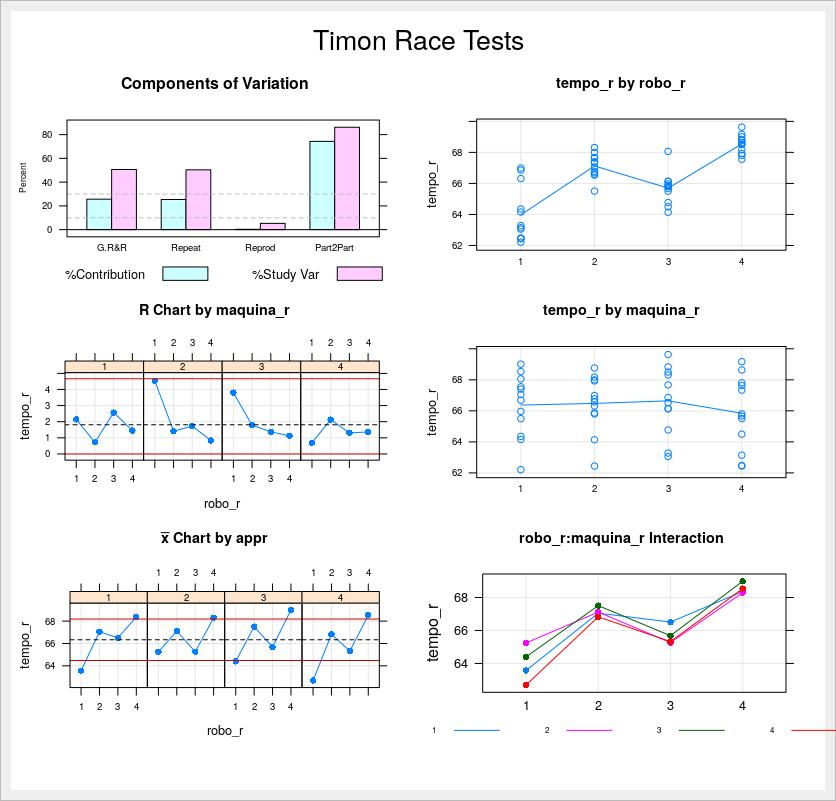
\includegraphics[scale=0.8]{images/timon_race_tests.png}
    \legend{Fonte: Autoria própria.}
\end{figure}

Pode-se observar na (tempo\_r by robo\_r) que robô 4 apresenta um valor de tempo médio maior que os demais, isso ocorre, a priori, devido ao posicionamento do Aruco que sinaliza o fim de percurso da simulação. Também podemos observar em x\_chart by appr que as 4 máquinas apresentarem comportamentos similares na coleta de dados, porém com amplitudes diferentes, o que indica possíveis falhas.

De acordo com a Figura 2, o p valor encontrado é maior que alpha, o que caracteriza uma distribuição normal nos resultados encontrados. Além disso, observa-se um valor de categorias distintas igual a 2 e, como pode ser observado também na Figura 1, maior contribuição vinculada ao item Part-To-Part, elementos considerados positivos para o sistema.

	\chapter{CONCLUSÃO}
\label{chap:conclusion}

A alta contribuição da Repetibilidade aliada à quase nula contribuição da Reprodutibilidade indica que o nosso sistema de medição apresenta alguma falha. Os fatos exibidos nos levam a concluir que um dos operadores responsáveis cometeu algum erro no momento dos testes, desta forma o sistema de medição apresentado não é considerado válido, sendo necessária uma nova coleta para novas análises.
	% \include{sections/03desenvolvimento}
	% \include{sections/04resultados}
	% \include{sections/05confiabilidade}
	% \include{sections/06conhecimento}
	% \include{sections/07conclusao}
	%\include{sections/02referencial}
	%\include{sections/03metodo}
% --------------------------------------------------------------------------
% Referências
	% \cleardoublepage
	% \titleformat{\chapter}[display]{\vspace*{-24pt}\ABNTEXchapterfont\large\bfseries}{\chaptertitlename\ \thechapter}{12pt}{\Large}
	% \bibliography{bibliography}
% --------------------------------------------------------------------------
% % Apêndices
% 	\apendices
% 	\justify
% 	%
% 	\chapter{Questões de abordagem à pesquisa}
% 	\label{apend:quest}
% 	%\includepdf[pages={{},-}]{appendix/listquest.pdf}
% 	\lipsum[1] % Comentar e adicionar apêndice aqui
% 	%
% 	\chapter{Um assunto importante}
% 	\label{apend:assunto}
% 	\lipsum[1] % Comentar e adicionar apêndice aqui
	

% --------------------------------------------------------------------------
% % Anexos                                                                     
% 	\anexos
% 	\justify
% 	%
% 	\chapter{Outro assunto importante}
% 	\label{ann:relant}
% 	%\includepdf[pages={{},-}]{annex/manisubanterioridade.pdf}
% 	\lipsum[1] % Comentar e adicionar apêndice aqui
% 	%
\end{document} 